% Flows to Words: Does the Encoding Matter? -- report (see report/outline.md for what goes in each section).
% Format: ACL two-column style (acl.sty + acl_natbib.bst, unmodified copies from github.com/acl-org/acl-style-files).
% Page limit: 7 pages of main text at most (abstract to Conclusion); Limitations, references and appendix do not count.
% To stay under it, the main text keeps only the tables the argument needs; every other table/figure is in the appendix.
%
% RULE: never type a result or setting into this file. Every number comes from generated/numbers_*.tex:
%   \res{key}          prints a value, e.g. \res{exp2.xgboost.none.nf_unsw_nb15.macro_f1}
%   \resnum{key}       the raw number (for arithmetic)
%   \resdiff{a}{b}     a - b, rounded (needs LaTeX 2022 or newer for \fpeval; Overleaf has it)
%   \respct{a}{b}      100 * a / b, rounded (a share in %, e.g. rows removed by dedupe)
%   \resor{key}{text}  the value, or `text` (no warning) if the key has none yet; the generated tables use it
%   \respercentof{key} a fraction key as a percentage (e.g. the 0.7 train split -> 70)
% A key without a value prints a red ?? plus the key and a warning in the log. All keys and their current values:
% results/numbers_analysis.md and results/numbers_privacy*.md in the code repo.
%
% Everything under generated/ (tables, figures, numbers) is written by `uv run ftw analysis privacy privacy_edge`; do
% not edit it here or on Overleaf. This folder (report/) is the Overleaf project, synced with git subtree.
% Sentences whose wording depends on a verdict carry a "% CHECK <key>" comment: re-read them after a rerun.
% Citations: \cite or \citep = "(Author, Year)", \citet = "Author (Year)" when the authors are part of the sentence.
\documentclass[11pt]{article}
\usepackage[final]{acl}

% ---- fonts (as in the ACL template) ----
\usepackage{times}
\usepackage{latexsym}
\usepackage[T1]{fontenc}
\usepackage[utf8]{inputenc}
\usepackage{microtype}
\usepackage{inconsolata}                    % typewriter font for hashes and key=value text

% ---- tables, figures, lists ----
\usepackage{booktabs}
\usepackage{graphicx}
\usepackage{amsmath}
\usepackage{xfp}                            % \fpeval on older LaTeX (e.g. tectonic); built in since 2022
\usepackage{xcolor}
\usepackage{enumitem}
\usepackage{tikz}
\usetikzlibrary{positioning, arrows.meta}
\usepackage[most]{tcolorbox}
\usepackage{float}                           % [H]: appendix figures stay under their heading
\usepackage{cleveref}                       % after hyperref, which acl.sty loads

% ---- colours of the pipeline figure (blue ramp of the generated figures) ----
\definecolor{accent}{HTML}{184F95}
\definecolor{accentlight}{HTML}{CDE2FB}

% "Key findings" box in the introduction
\newtcolorbox{findings}[1][]{enhanced, colback=white, colframe=black, boxrule=0.4pt, arc=0pt,
  left=4pt, right=4pt, top=3pt, bottom=3pt, coltitle=black, colbacktitle=white, fonttitle=\bfseries, title=#1}

\graphicspath{{generated/figures/}}
\newcommand{\todo}[1]{\textcolor{red}{[TODO: #1]}}

% ---- generated numbers ----
\makeatletter
\newcommand{\resset}[3]{\expandafter\def\csname res@#1\endcsname{#2}\expandafter\def\csname resraw@#1\endcsname{#3}}
\DeclareRobustCommand{\res}[1]{%
  \ifcsname res@#1\endcsname\csname res@#1\endcsname
  \else\@latex@warning{No generated value for result key `#1'}\textcolor{red}{\textbf{??}\texttt{\detokenize{#1}}}\fi}
\DeclareRobustCommand{\resor}[2]{\ifcsname res@#1\endcsname\csname res@#1\endcsname\else #2\fi}
\newcommand{\resnum}[1]{\ifcsname resraw@#1\endcsname\csname resraw@#1\endcsname\else 0\fi}
\newcommand{\resdiff}[2]{\fpeval{round(\resnum{#1}-\resnum{#2},\resdecimals)}}
\newcommand{\respercentof}[1]{\fpeval{round(100*\resnum{#1},\respctdecimals)}}
\newcommand{\respct}[2]{\fpeval{round(100*\resnum{#1}/\resnum{#2},\respctdecimals)}}
\makeatother
\newcommand{\resinput}[1]{\IfFileExists{generated/#1.tex}{\input{generated/#1.tex}}{\typeout{Missing generated/#1.tex}}}
\resinput{numbers_analysis}
\resinput{numbers_privacy}
\resinput{numbers_privacy_edge}
\newcommand{\gentable}[1]{\resizebox{\linewidth}{!}{\input{generated/#1.tex}}}

% ---- title and authors ----
\title{Flows to Words: Does the Encoding Matter?\thanks{Course project, T-725-MALV Natural Language Processing,
  Reykjavik University, Fall 2026. Supervisor: Stefán Ólafsson.}}

\author{Daniel Z. El Deen K. Al Hennaw \\ Reykjavik University \\ \texttt{daniele23@ru.is} \And
  Tim Liebhaber \\ Reykjavik University \\ \texttt{tim.liebhaber@uni-ulm.de} \And
  Vid Kali\v{s}nik \\ Reykjavik University \\ \texttt{vid26@ru.is}}

\begin{document}
% The text is in sections/ (one file per section); this file holds the setup and the order of the sections.
\maketitle

%====== MAIN TEXT (7-page limit) ======%
\begin{abstract}
\noindent Language models are increasingly used for network intrusion detection. To use them, each flow record is
first turned into text. SecurityBERT, for example, hashes every \texttt{column\$value} pair (PPFLE) and reports
\res{exp1.paper.accuracy} accuracy on Edge-IIoTset. We ask how much this choice of encoding matters. We compare four
encodings: raw PPFLE, PPFLE on quantile bins, \texttt{key=value} text and a sentence template. Each is paired with a
small BERT trained from scratch and with a pretrained DistilBERT, and all are compared with a tuned XGBoost on four
NetFlow datasets and Edge-IIoTset, both within and across datasets. The published Edge-IIoTset result turns out to
depend on a label leak, because empty fields are spelled differently in normal and attack traffic. Within a dataset,
XGBoost is as good as or better than every text model. Across datasets, binning the values before hashing transfers
best for both language models. Finally, a dictionary attack reverses
\res{privacy.e1_ppfle.public.token_share.min}--\res{privacy.e1_ppfle.public.token_share.max}\,\% of the PPFLE tokens
in the NetFlow test sets and \res{privacy_edge.edge_iiotset_raw.e1_ppfle.bruteforce.token_share}\,\% on
Edge-IIoTset, so the encoding does not protect the data.
% CHECK hyp.H2.verdict, hyp.H3.verdict
\end{abstract}

\section{Introduction}\label{sec:intro}
Network intrusion detection systems (NIDS) look at network flows and decide whether each one is benign or one of
several attack types. A flow is a single row of summary statistics for one connection. Recent work feeds such rows to
language models by writing them out as text~\cite{hegselmann2022tabllm,borisov2022great}.
SecurityBERT~\cite{ferrag2024securitybert} goes one step further. Its Privacy-Preserving Fixed-Length Encoding (PPFLE)
replaces each \texttt{column\$value} pair with a truncated hash, and a small BERT~\cite{devlin2019bert} is trained on
the resulting tokens. The paper reports \res{exp1.paper.accuracy} accuracy on the \res{nclasses.edge_iiotset}-class
Edge-IIoTset~\cite{ferrag2022edge} and claims that the hashes protect the raw values.

Three questions remain open. First, the encoding itself is never tested. Hashing removes both the numeric order and
any English meaning, and it is unclear whether a readable encoding would do better. Second, the baselines were weak.
On tabular data, a tuned gradient-boosted tree is the natural competitor. Third, real deployments meet networks they
were not trained on, and the privacy claim has never been checked. We therefore ask:
\begin{description}[leftmargin=3.2em, labelwidth=2.6em, font=\bfseries]
  \item[RQ1] Does the PPFLE + small BERT result reproduce on Edge-IIoTset?
  \item[RQ2] Within one dataset, how do four encodings compare with each other and with XGBoost?
  \item[RQ3] When a model is trained on one dataset and tested on another, which encoding generalises best?
  \item[RQ4] Is PPFLE actually privacy-preserving?
\end{description}
We also test four hypotheses:
\begin{description}[leftmargin=3.2em, labelwidth=2.6em, font=\bfseries, itemsep=0pt]
  \item[H1] PPFLE does well within a dataset.
  \item[H2] XGBoost is as good or better within a dataset.
  \item[H3] Readable or binned encodings transfer better than raw PPFLE.
  \item[H4] A pretrained model benefits from readable encodings, but not from hashes.
\end{description}

We make four contributions. We run a controlled benchmark of encodings and language models against XGBoost
(\cref{sec:results}). We find a label leak in Edge-IIoTset that explains the published accuracy (\cref{sec:leak}). We
show that a simple dictionary attack reverses most PPFLE tokens (\cref{sec:privacy}). Finally, we discuss when the NLP
route pays off (\cref{sec:discussion}). The box below gives the short answers.

\begin{findings}[Key findings]
\begin{description}[leftmargin=3.2em, labelwidth=2.6em, font=\bfseries, itemsep=2pt]
  \item[RQ1] The published accuracy reproduces, but only because of a label leak. PPFLE + small BERT reaches
    \res{exp1.bert_small.e1_ppfle.edge_iiotset_raw.multiclass.accuracy} on the data as published (paper:
    \res{exp1.paper.accuracy}) and \res{exp1.bert_small.e1_ppfle.edge_iiotset.multiclass.accuracy} once the leak is
    removed.
  \item[RQ2] XGBoost is as good as or better than every text model on every dataset (H2: \res{hyp.H2.verdict}).
    Raw PPFLE is never the best encoding (H1: \res{hyp.H1.verdict}).
  \item[RQ3] Binning before hashing transfers best. For the small BERT, off-diagonal macro-F1 rises from
    \res{exp3.bert_small.e1_ppfle.off.macro_f1} to \res{exp3.bert_small.e2_ppfle_bins.off.macro_f1}, and DistilBERT
    with binned PPFLE is the best method overall at \res{exp3.distilbert.e2_ppfle_bins.off.macro_f1} (H3:
    \res{hyp.H3.verdict}). Within a dataset, pretraining helps on readable text. Across datasets it helps on
    hashes instead (H4: \res{hyp.H4.verdict}).
  \item[RQ4] PPFLE is not private. A dictionary attack reverses
    \res{privacy.e1_ppfle.public.token_share.min}--\res{privacy.e1_ppfle.public.token_share.max}\,\% of the NetFlow
    test tokens and \res{privacy_edge.edge_iiotset_raw.e1_ppfle.bruteforce.token_share}\,\% on Edge-IIoTset.
\end{description}
\end{findings}
% CHECK hyp.H1-H4 verdicts and the E2 ranking in exp3_cross

\section{Related work}\label{sec:related}
\paragraph{Tables as text.} When table rows are written out as text, pretrained language models can classify tabular
data~\cite{hegselmann2022tabllm} and even generate realistic new rows~\cite{borisov2022great}. These works use
readable \texttt{column is value} templates. They do not study hashed or binned encodings, and they do not test
transfer between datasets.

\paragraph{Language models for intrusion detection.} SecurityBERT and PPFLE~\cite{ferrag2024securitybert} were
evaluated on Edge-IIoTset~\cite{ferrag2022edge} against classical baselines. Edge-IIoTset is a testbed dataset of
IoT/IIoT traffic with \res{nclasses.edge_iiotset} classes, benign plus several attack types. Large language models
that only receive a prompt with the flow record stay well below tree models~\cite{flows2words2025}.
\citet{edgeleak2026} independently found the placeholder-spelling artifact in Edge-IIoTset that we analyse in
\cref{sec:leak}.

\paragraph{Datasets and baselines.} The NetFlow datasets of \citet{sarhan2021netflow} describe
several public NIDS datasets with one shared feature set, which makes cross-dataset evaluation possible \citep{uqnids}. We use
XGBoost~\cite{chen2016xgboost} as the tabular baseline and DistilBERT~\cite{sanh2019distilbert} as the pretrained
language model. Our small BERT uses byte-level byte-pair encoding~\cite{sennrich2016bpe} as its tokenizer.

\section{Data}\label{sec:data}
\paragraph{NetFlow datasets.} We use the v3 release of NF-UNSW-NB15, NF-ToN-IoT, NF-BoT-IoT and NF-CSE-CIC-IDS2018,
which all share one feature set. We drop \res{cfg.data.columns.leaky.count} identifier columns that would let a model
memorise hosts or time instead of behaviour: the IP addresses, the source port, the flow timestamps and the DNS query
id. The destination port is kept. This leaves \res{cfg.data.columns.features.count} features.

From each dataset we draw a stratified sample of \res{cfg.data.sampling.sample_size} flows. Classes with fewer than
\res{cfg.data.sampling.rare_class_threshold} flows are kept whole. NF-BoT-IoT is almost entirely attack traffic, so it
keeps all of its benign flows. After the identifier columns are gone, we remove exact duplicates and flows that have
identical features but different labels. Each sample is then split
\respercentof{cfg.data.split.train}/\respercentof{cfg.data.split.val}/\respercentof{cfg.data.split.test} into train,
validation and test sets, stratified by class (sizes in \cref{tab:data}, \cref{app:data}).

\paragraph{Edge-IIoTset.} We use the published ``DNN'' file and drop the same
\res{cfg.data_edge.columns.leaky.count} columns that the dataset authors drop (addresses, ports, payloads and
timestamps). This leaves \res{cfg.data_edge.columns.features.count} features. Sampling, deduplication and splitting
follow the NetFlow procedure.


\paragraph{Leakage check.} Before modelling, we train XGBoost on each feature alone (train $\to$ validation) and
look closely at any feature that separates the classes by itself. In NF-UNSW-NB15, the minimum TTL alone reaches
binary macro-F1 \res{leakage.nf_unsw_nb15.binary.MIN_TTL}, and the maximum TTL reaches
\res{leakage.nf_unsw_nb15.binary.MAX_TTL}. The reason is that all attack traffic comes from one subnet and all benign
traffic from another, so the TTL and packet-size fingerprints of these machines give the label away. In the
multiclass task the same feature reaches only \res{leakage.nf_unsw_nb15.multiclass.MIN_TTL}, because all attack
classes share the same attacker hosts. We keep all features and treat the binary within-dataset results on
NF-UNSW-NB15 as saturated.

\section{A label leak in Edge-IIoTset}\label{sec:leak}
In the published Edge-IIoTset files, an empty field is written as \texttt{"0"} in the normal-traffic captures and as
\texttt{"0.0"} in the attack captures. \citet{edgeleak2026} reports the same artifact. The spelling alone
therefore reveals the label. On the data as published, four single features reach binary macro-F1
\res{leakage.edge_iiotset_raw.binary.mqtt.topic}: \texttt{mqtt.topic}, \texttt{mqtt.protoname},
\texttt{mqtt.conack.flags} and \texttt{dns.qry.name.len}. Once the spelling is unified, the best of them reaches only
\res{leakage.edge_iiotset.binary.dns.qry.name.len}. Any model that sees the raw strings can exploit this. That
includes PPFLE, because \texttt{column\$0} and \texttt{column\$0.0} hash to different tokens.

The effect is large (\cref{tab:exp1}). XGBoost reaches \res{exp1.xgboost.none.edge_iiotset_raw.multiclass.accuracy}
accuracy on the data as published, but \res{exp1.xgboost.none.edge_iiotset.multiclass.accuracy} after the fix. Its
binary macro-F1 drops from \res{exp1.xgboost.none.edge_iiotset_raw.binary.macro_f1} to
\res{exp1.xgboost.none.edge_iiotset.binary.macro_f1}. Our PPFLE + small BERT replication shows the same pattern. It
reaches \res{exp1.bert_small.e1_ppfle.edge_iiotset_raw.multiclass.accuracy} accuracy on the data as published, close
to the paper's \res{exp1.paper.accuracy}, but only \res{exp1.bert_small.e1_ppfle.edge_iiotset.multiclass.accuracy} on
the fixed data. All other Edge-IIoTset results in this report use the fixed data. We also noticed that the columns
\texttt{dns.qry.name} and \texttt{dns.qry.name.len} seem to be swapped in the raw file. We keep them as published.

\section{Method}\label{sec:method}
\Cref{fig:pipeline} (\cref{app:data}) gives an overview. Every method sees the same cleaned, deduplicated and split data. The language
models read it through one of four text encodings, while XGBoost reads the table directly.


\paragraph{Encodings.} All encodings go through the features in the same fixed order, write missing values as
\texttt{NA} and join the parts with spaces (\cref{tab:examples}).
\textbf{E1 (PPFLE)} replaces each \texttt{column\$value} with its \res{cfg.encoders.hash.algorithm} hash, cut to
\res{cfg.encoders.hash.length} hexadecimal characters, as in SecurityBERT.
\textbf{E2 (binned PPFLE)} first maps each numeric value to one of \res{cfg.encoders.binning.n_bins} quantile bins,
fitted on the training split, and then hashes \texttt{column\$binK}. Categorical columns such as ports, protocols and
flags are hashed as in E1. \textbf{E3} writes readable \texttt{key=value} pairs with short column names. \textbf{E4}
fills a fixed template of English sentences and replaces protocol codes with their names.

\begin{table*}[!tbp]
  \centering
  \caption{The same NetFlow flow in the four encodings (beginning of each text only).}
  \label{tab:examples}
  % One flow in every encoding: generated by src/eval/analysis.py from results/encoding_stats.json, do not edit.
\begin{tabular}{@{}l p{0.78\linewidth}@{}}
\toprule
Encoding & Text \\
\midrule
E1 PPFLE & \texttt{\small e61bda9819b7fb55 4fbfe692dd218a7c 49f8efc3a07a7d29 46928dd8ca3a3f99 99a76dcb3e29cf31 da597cc9203f6df4 3efb85bbd25efb1a ece41bff11d60b21 3240b9e49a543820 fa2e50ac5f639e3f babb86cc04e6de22 c9436fb79e324b5e 0fce18341c7620a7 \dots} \\
E2 PPFLE-bins & \texttt{\small e61bda9819b7fb55 4fbfe692dd218a7c 49f8efc3a07a7d29 7fc09090edd30595 02e02bf5a981da22 37d4af979005d2cb 29fde00e2ab18ffe ece41bff11d60b21 3240b9e49a543820 fa2e50ac5f639e3f 34da606c4a74c86b 5b3a60bc305317a0 1126843ce2916164 \dots} \\
E3 key=value & \texttt{\small dst port=31992 proto=6 app proto=11.0 in bytes=4704 in pkts=28 out bytes=2976 out pkts=28 tcp flags=27 client flags=27 server flags=27 duration=335 in duration=334 out duration=334 min ttl=31 max ttl=32 longest pkt=984 shortest \dots} \\
E4 sentence & A TCP flow with application protocol NFS to destination port 31992 lasted 335 milliseconds. The client sent 28 packets (4704 bytes) over 334 milliseconds, and the server replied with 28 packets (2976 bytes) over 334 milliseconds. \dots \\
\bottomrule
\end{tabular}

\end{table*}

\paragraph{Models.} \textbf{XGBoost}, an ensemble of gradient-boosted decision trees, reads the cleaned table
directly. Its depth, learning rate and class weighting are chosen on the validation split, with early stopping.

Both language models are BERT-style Transformer encoders~\cite{devlin2019bert}. They read the token sequence of a
flow, and a classification layer on the representation of the first token predicts the class. The \textbf{small
BERT} starts from random weights and only ever sees flow texts. It follows the size stated for SecurityBERT: \res{cfg.bert_small.model.num_hidden_layers}
layers, hidden size \res{cfg.bert_small.model.hidden_size}, \res{cfg.bert_small.model.num_attention_heads} attention
heads and feed-forward size \res{cfg.bert_small.model.intermediate_size}. This gives \res{params.bert_small.millions}\,M
parameters, not the \res{exp1.paper.params_millions}\,M the paper states. It uses a byte-level BPE tokenizer with
\res{cfg.bert_small.tokenizer.vocab_size} tokens, trained separately for each encoding on the training split. The
maximum input length covers the \res{cfg.bert_small.tokenizer.coverage_percentile}th percentile of training rows. The
model is trained for \res{cfg.bert_small.training.epochs} epochs, and we keep the epoch that does best on validation.

\textbf{DistilBERT}~\cite{sanh2019distilbert} is a compressed version of BERT. It has half the layers of BERT-base and
was trained by knowledge distillation, that is, to reproduce BERT's predictions on the same English text (books and
Wikipedia). It keeps most of BERT's accuracy on language-understanding benchmarks while being smaller and faster.
Unlike the small BERT, it therefore starts with knowledge of English words and numbers, which is what H4 tests. We
fine-tune the pretrained uncased model (\res{params.distilbert.millions}\,M parameters) for
\res{cfg.distilbert.training.epochs} epochs with its own WordPiece tokenizer, which is not retrained. Hashes break into many WordPieces, so E1
needs \res{encoding.stats.nf_unsw_nb15.encodings.e1_ppfle.wordpiece_tokens.p99} tokens for nearly all rows. It is
therefore cut at DistilBERT's limit of \res{cfg.distilbert.tokenizer.max_len_cap} tokens. Side runs with shorter
hashes, where nothing is cut, show no systematic cost of this truncation (\cref{tab:side}, \cref{app:more}).

\paragraph{Tuning and protocol.} The learning rate of each language model is picked from a grid of
\res{cfg.bert_small.tuning.lr_grid.count} values on the validation split of one pilot dataset, NF-UNSW-NB15, and
reused for the other NetFlow datasets. Edge-IIoTset is tuned the same way on its own validation split.
% CHECK cfg.<model>.tuning.pilot.dataset and cfg.<model>_edge.tuning.pilot.dataset
Every method sees the same samples, splits and columns, and the test split is used only once. Every model is run
with \res{seeds.distilbert} seeds and reported as mean $\pm$ standard deviation. DistilBERT is the most expensive
model, so its second and third seeds were trained on an A100 GPU of the Elja cluster, with the same settings and
learning rates as the first. Only the two truncation side runs use a single seed.
% CHECK seeds.xgboost = seeds.bert_small = seeds.distilbert

Macro-F1 is our main metric. We also report accuracy, to compare with the paper, and for cross-dataset runs the
attack recall and false-positive rate (FPR). For the hypotheses, we treat two numbers as different only if they
differ by more than \res{cfg.analysis.hypotheses.tie_margin} and by more than the larger of their seed standard
deviations. Otherwise we call them tied. We call an encoding ``good'' if it is within
\res{cfg.analysis.hypotheses.well_margin} of the best method.


\section{Results}\label{sec:results}

\subsection{Experiment 1: replication (RQ1)}
\begin{table*}[!tbp]
  \centering
  \caption{Edge-IIoTset, test set: data as published vs.\ with the placeholder spelling unified (``--'': not run).}
  \label{tab:exp1}
  \gentable{exp1_replication}
\end{table*}
On the data as published, PPFLE + small BERT reaches
\res{exp1.bert_small.e1_ppfle.edge_iiotset_raw.multiclass.accuracy} accuracy, against the paper's
\res{exp1.paper.accuracy}. The number therefore reproduces (RQ1: \res{hyp.RQ1.verdict}).
% CHECK hyp.RQ1.verdict
As \cref{sec:leak} shows, however, it only reproduces because of the leak. On the fixed data the same model reaches
\res{exp1.bert_small.e1_ppfle.edge_iiotset.multiclass.accuracy} accuracy and
\res{exp1.bert_small.e1_ppfle.edge_iiotset.multiclass.macro_f1} macro-F1. A plain XGBoost does better, with
\res{exp1.xgboost.none.edge_iiotset.multiclass.accuracy} accuracy and
\res{exp1.xgboost.none.edge_iiotset.multiclass.macro_f1} macro-F1.

\subsection{Experiment 2: within-dataset benchmark (RQ2, H1, H2)}
\begin{table*}[!tbp]
  \centering
  \caption{Test macro-F1 (multiclass), mean $\pm$ std over \res{seeds.distilbert} seeds.}
  \label{tab:exp2}
  \gentable{exp2_within_macro_f1}
\end{table*}
\Cref{tab:exp2} shows the within-dataset results (as a chart: \cref{fig:exp2}, \cref{app:more}). XGBoost is as good as or better than every text model on
every dataset (H2: \res{hyp.H2.verdict}, \res{hyp.H2.held} of \res{hyp.H2.total} datasets). On NF-UNSW-NB15 it leads
the best text model by \resdiff{exp2.xgboost.none.nf_unsw_nb15.macro_f1}{exp2.distilbert.e3_kv.nf_unsw_nb15.macro_f1}
macro-F1, and on NF-BoT-IoT by
\resdiff{exp2.xgboost.none.nf_bot_iot.macro_f1}{exp2.distilbert.e3_kv.nf_bot_iot.macro_f1}, just above our tie
margin. On NF-ToN-IoT the best
text model comes within our tie margin. On NF-CSE-CIC-IDS2018, DistilBERT with E3 is even slightly ahead
(\resdiff{exp2.distilbert.e3_kv.nf_cse_cic_ids2018.macro_f1}{exp2.xgboost.none.nf_cse_cic_ids2018.macro_f1}), but
that is still a tie.

On Edge-IIoTset (fixed data), XGBoost reaches \res{exp2.xgboost.none.edge_iiotset.macro_f1}. The best small BERT
(\res{best.edge_iiotset.bert_small.encoding}) reaches \res{best.edge_iiotset.bert_small.value}, and DistilBERT with
\res{best.edge_iiotset.distilbert.encoding} reaches \res{best.edge_iiotset.distilbert.value}. That is the highest
value in the column, but its lead over XGBoost
(\resdiff{best.edge_iiotset.distilbert.value}{exp2.xgboost.none.edge_iiotset.macro_f1}) is within the tie margin.
% CHECK hyp.H2.verdict and its per-dataset checks in results/analysis_summary.md, best.<d>.method (NF-CSE-CIC-IDS2018
% and Edge-IIoTset: DistilBERT E3), best.nf_unsw_nb15.distilbert.encoding

For DistilBERT, readable key=value text (E3) is the best encoding on every dataset, with the sentence template (E4)
usually close behind. For the small BERT, the best encoding changes from dataset to dataset. Raw PPFLE is never the
best encoding for either model and is usually among the weakest. Its best model is within
\res{cfg.analysis.hypotheses.well_margin} of the best method on only \res{hyp.H1.held} of \res{hyp.H1.total}
datasets (H1: \res{hyp.H1.verdict}). Seed variance also matters. On NF-CSE-CIC-IDS2018, the small BERT with E1 varies
by $\pm$\res{exp2.bert_small.e1_ppfle.nf_cse_cic_ids2018.macro_f1.std} between seeds, which is enough to change the
order of the encodings.
% CHECK hyp.H1.verdict; best.<d>.distilbert.encoding = E3 on all five datasets; E1 never ranks first

\paragraph{Error analysis.} Most of the errors come from a few classes (\cref{app:errors}). On NF-UNSW-NB15, the
\texttt{generic} class is hard for every method. XGBoost reaches a per-class F1 of
\res{perclass.xgboost.none.nf_unsw_nb15.generic} on it, and the small BERT with E1 only
\res{perclass.bert_small.e1_ppfle.nf_unsw_nb15.generic}. The rare \texttt{worms} class is found by XGBoost
(\res{perclass.xgboost.none.nf_unsw_nb15.worms}) and by DistilBERT with E3
(\res{perclass.distilbert.e3_kv.nf_unsw_nb15.worms}), but the small BERT with E1 misses it
(\res{perclass.bert_small.e1_ppfle.nf_unsw_nb15.worms}). On NF-CSE-CIC-IDS2018, every method labels most
\texttt{infiltration} flows as benign (XGBoost:
\res{confusion.xgboost.none.nf_cse_cic_ids2018.infiltration.benign}\,\%). This suggests that these flows cannot be told
apart from benign traffic using the NetFlow features. On Edge-IIoTset, no class stays below a per-class F1 of
\res{cfg.analysis.errors.hard_class_f1} for every method. The strongest methods (XGBoost, DistilBERT with E3 or E4, and the
small BERT with E4) all make the same mistakes: application-layer attacks that look like benign traffic. XGBoost,
for example, labels
\res{confusion.xgboost.none.edge_iiotset.ddos_http.benign}\,\% of \texttt{ddos\_http} flows and
\res{confusion.xgboost.none.edge_iiotset.uploading.benign}\,\% of \texttt{uploading} flows as benign. With binned
PPFLE (E2), both language models instead confuse attack classes with each other, for example \texttt{uploading} with
\texttt{password}, probably because the bins merge values that would separate these attacks.
% CHECK hard.edge_iiotset and the top mix-ups per method (computed from results/run_details)

\subsection{Experiment 3: cross-dataset transfer (RQ3, H3)}
\begin{table*}[!tbp]
  \centering
  \caption{Mean over the \res{exp3.n_datasets}$\times$\res{exp3.n_datasets} grid: same dataset (diagonal) vs.\
    transfer (off-diagonal).}
  \label{tab:exp3}
  \gentable{exp3_cross}
\end{table*}
When a model is trained and tested on the same dataset, every method detects attacks almost perfectly. XGBoost, for
example, reaches a diagonal macro-F1 of \res{exp3.xgboost.none.diag.macro_f1}. Transfer to another dataset is much
harder (\cref{tab:exp3}; all pairs: \cref{fig:exp3}, \cref{app:more}). The average off-diagonal macro-F1 of XGBoost is only
\res{exp3.xgboost.none.off.macro_f1}, and some pairs collapse completely. XGBoost trained on NF-CSE-CIC-IDS2018 and
tested on NF-BoT-IoT reaches just \res{exp3.xgboost.none.nf_cse_cic_ids2018.nf_bot_iot.macro_f1}.

Binning helps both language models. With E2 instead of E1, the small BERT improves from
\res{exp3.bert_small.e1_ppfle.off.macro_f1} to \res{exp3.bert_small.e2_ppfle_bins.off.macro_f1}, and DistilBERT from
\res{exp3.distilbert.e1_ppfle.off.macro_f1} to \res{exp3.distilbert.e2_ppfle_bins.off.macro_f1}. That is the highest
off-diagonal score of any method. Readable text (E3, E4) helps the small BERT but not DistilBERT (H3:
\res{hyp.H3.verdict}). For DistilBERT, both readable encodings even
transfer worse than raw PPFLE (\res{exp3.distilbert.e3_kv.off.macro_f1} and
\res{exp3.distilbert.e4_sentence.off.macro_f1} against \res{exp3.distilbert.e1_ppfle.off.macro_f1}). DistilBERT with E2 also catches more attacks
than XGBoost, with an attack recall of \res{exp3.distilbert.e2_ppfle_bins.off.attack_recall} against
\res{exp3.xgboost.none.off.attack_recall}, at a similar false-positive rate
(\res{exp3.distilbert.e2_ppfle_bins.off.fpr} against \res{exp3.xgboost.none.off.fpr}; \cref{app:more}).
% CHECK hyp.H3.verdict and the E2 ranking in exp3_cross

\subsection{Does pretraining help readable encodings? (H4)}
H4 predicts that DistilBERT beats the small BERT on readable encodings only. The data show gains on readable text,
for example \resdiff{exp2.distilbert.e3_kv.nf_unsw_nb15.macro_f1}{exp2.bert_small.e3_kv.nf_unsw_nb15.macro_f1}
macro-F1 for E3 on NF-UNSW-NB15. But they also show gains on hashes, for example
\resdiff{exp3.distilbert.e2_ppfle_bins.off.macro_f1}{exp3.bert_small.e2_ppfle_bins.off.macro_f1} off-diagonal
macro-F1 for E2 (H4: \res{hyp.H4.verdict}). So pretraining helps beyond reading English, but not everywhere. On
Edge-IIoTset both models score the same on hashes, \res{exp2.distilbert.e1_ppfle.edge_iiotset.macro_f1} against
\res{exp2.bert_small.e1_ppfle.edge_iiotset.macro_f1} for E1 and
\res{exp2.distilbert.e2_ppfle_bins.edge_iiotset.macro_f1} against
\res{exp2.bert_small.e2_ppfle_bins.edge_iiotset.macro_f1} for E2, while DistilBERT does gain on readable text. Model
size is a confounder here (\res{params.distilbert.millions}\,M against \res{params.bert_small.millions}\,M
parameters). A larger model that starts from pretrained weights may simply fit token statistics better.
Across datasets the pattern even reverses. There, DistilBERT gains on hashes
(\res{exp3.distilbert.e1_ppfle.off.macro_f1} against \res{exp3.bert_small.e1_ppfle.off.macro_f1} for E1) but not on
readable text (\res{exp3.distilbert.e3_kv.off.macro_f1} against \res{exp3.bert_small.e3_kv.off.macro_f1} for E3, and
\res{exp3.distilbert.e4_sentence.off.macro_f1} against \res{exp3.bert_small.e4_sentence.off.macro_f1} for E4).
% CHECK hyp.H4.verdict and its cross-dataset checks (E1/E2 gain, E3/E4 no gain)

\subsection{Experiment 4: is PPFLE private? (RQ4)}\label{sec:privacy}
\begin{table*}[!tbp]
  \centering
  \caption{Dictionary attack on the NetFlow test splits: share of tokens and of whole rows recovered (cumulative
    levels).}
  \label{tab:privacy}
  \gentable{privacy_attack}
\end{table*}
PPFLE uses an unsalted hash. Anyone who knows the scheme can therefore hash candidate values and compare them with
the tokens. Our attacker knows the scheme and the public NetFlow feature list (column names and types), but not the
data. The attack runs in three cumulative steps (\cref{tab:privacy}; \cref{fig:privacy}, \cref{app:privacy}).

First, we try every possible value of the \res{privacy.n_low_cardinality} low-cardinality columns, such as ports,
protocols, TCP flags, TTLs and application codes. This alone reverses
\res{privacy.e1_ppfle.enumerate.token_share.min}--\res{privacy.e1_ppfle.enumerate.token_share.max}\,\% of all E1
tokens. Second, we try every whole number up to \res{privacy.bruteforce.max} for the remaining numeric columns. This
raises the share to
\res{privacy.e1_ppfle.bruteforce.token_share.min}--\res{privacy.e1_ppfle.bruteforce.token_share.max}\,\% and already
recovers many whole rows exactly, for example \res{privacy.nf_cse_cic_ids2018.e1_ppfle.bruteforce.row_share}\,\% of
the NF-CSE-CIC-IDS2018 test flows. Third, we add a dictionary of the values seen in the other public datasets. Token
recovery then reaches \res{privacy.e1_ppfle.public.token_share.min}--\res{privacy.e1_ppfle.public.token_share.max}\,\%,
and full rows reach \res{privacy.nf_cse_cic_ids2018.e1_ppfle.public.row_share}\,\% on NF-CSE-CIC-IDS2018 and
\res{privacy.nf_ton_iot.e1_ppfle.public.row_share}\,\% on NF-ToN-IoT. The values that resist are fractional
bytes-per-second rates and very large throughput counters (\cref{fig:privacycols}, \cref{app:privacy}).

E2 is even easier to attack. Every binned column has only \res{cfg.encoders.binning.n_bins} possible tokens, so
enumeration alone reverses \res{privacy.e2_ppfle_bins.enumerate.token_share.min}\,\% of the tokens. The attacker then
learns the bin, which is a quantile range, rather than the exact value. We checked every recovered token against the
true value.

The attack also works on SecurityBERT's own dataset (\cref{tab:privacyedge}, \cref{app:privacy}). There is no independent public dataset
with the same columns as Edge-IIoTset, so we only use the first two steps. The text columns are guessed from public
vocabularies (HTTP methods and versions, MQTT protocol names) plus the two empty-field spellings. On the data as
published, this reverses \res{privacy_edge.edge_iiotset_raw.e1_ppfle.bruteforce.token_share}\,\% of the PPFLE tokens
and \res{privacy_edge.edge_iiotset_raw.e1_ppfle.bruteforce.row_share}\,\% of whole rows. What stays hidden is mostly
the TCP sequence and acknowledgement numbers, whose values are larger than our brute-force range. Of the raw
acknowledgement numbers, for example, only \res{privacy_edge.col.e1_ppfle.bruteforce.tcp.ack_raw}\,\% are recovered.

Deterministic hashing of low-entropy fields is pseudonymisation, not privacy protection. A keyed hash (an HMAC with a
secret key) would block this dictionary attack. It would still reveal which values are equal, though, and the model
would still learn from exact values that rarely recur in another network.

\section{Discussion}\label{sec:discussion}
\paragraph{Does the encoding matter?} Yes, but not in the way PPFLE suggests. Within a dataset, the encoding can
change a language model's macro-F1 by a lot, up to
\resdiff{exp2.distilbert.e3_kv.edge_iiotset.macro_f1}{exp2.distilbert.e2_ppfle_bins.edge_iiotset.macro_f1} for
DistilBERT on Edge-IIoTset. With pretraining, readable key=value text is the best choice on every dataset, while raw
hashing never is. Still, no encoding lets a text model clearly beat XGBoost. Where DistilBERT with E3 is slightly
ahead, on NF-CSE-CIC-IDS2018 and Edge-IIoTset, the lead is within the tie margin. Across datasets, the encoding even
decides whether a language model can beat XGBoost at all. Binning the values before hashing gives the largest
improvement for both language models, while readable text only helps the model trained from scratch. A likely reason is that raw hashing
destroys the numeric order. A model then has to memorise exact values, and those rarely recur in another network. Bins
keep a coarse order and produce tokens that are shared across datasets.
% CHECK hyp.H2.verdict, hyp.H3.verdict, best.<d>.distilbert.encoding (E3 everywhere), largest DistilBERT encoding gap

\paragraph{When does the NLP route pay off?} For detection within one known network, it does not. XGBoost is just as
accurate and trains in about \res{time.xgboost.train.median_s}\,s per run on our laptop GPU. The small BERT needs
about \res{time.bert_small.train.median_min}\,min and DistilBERT about \res{time.distilbert.train.median_h}\,h (\res{time.distilbert.cluster.train.median_min}\,min
on an A100). The
only setting where a language model came out clearly ahead is transfer to an unseen network, with binned PPFLE and
pretraining. This is also the setting that matters most in practice. The lead holds over all \res{seeds.distilbert} seeds
(\res{exp3.distilbert.e2_ppfle_bins.off.macro_f1} against \res{exp3.xgboost.none.off.macro_f1}), but it is measured
on only \res{exp3.n_datasets} datasets.

\paragraph{What about PPFLE?} As published, PPFLE offers neither better accuracy nor privacy. Its headline result
depends on a label leak, raw hashing transfers worse than binned hashing for both models, and most of its tokens can be reversed in a few
minutes on a laptop.

\section{Conclusion}\label{sec:conclusion}
How a network flow is turned into text does matter, but not in the way the PPFLE paper suggests. The
\res{exp1.paper.accuracy} accuracy reported for PPFLE on Edge-IIoTset only reproduces because empty fields reveal the
label. Without the leak, a plain XGBoost does better. Within a dataset, XGBoost matches or beats every combination of
encoding and language model, and readable text works best for the pretrained model. Across datasets, binning the values before hashing transfers
best, and a pretrained model benefits from it. Finally, hashing does not protect the data, since a dictionary attack
reverses most PPFLE tokens. Future work should check the cross-dataset results on more datasets and test keyed or
learned encodings that offer both transfer and privacy.
% CHECK hyp.RQ1.verdict, hyp.H2.verdict, hyp.H3.verdict


%====== AFTER THE MAIN TEXT (not counted in the page limit) ======%
\section*{Limitations}\label{sec:limitations}
Each model was run with only \res{seeds.distilbert} seeds, and the small BERT results vary noticeably between seeds
on some datasets. Single cells, especially cross-dataset ones, should therefore be read with care. Learning rates were
tuned on one pilot dataset (one for NetFlow, and Edge-IIoTset on itself), not per dataset. Our small BERT is smaller
than the size the paper states. E1 and E2 are truncated for DistilBERT, although the side runs suggest this costs
little. We kept the host fingerprint in NF-UNSW-NB15 and used one sample per dataset. The training times mix
different power states of a laptop GPU and are only a rough guide. DistilBERT's second and third seeds ran on a
faster cluster GPU, so the times we compare come from the first seed of every model. Finally, the privacy attack on Edge-IIoTset has no
public-dictionary step, so its numbers are a lower bound.

\section*{Acknowledgments}
Computer resources and research IT are provided by UTS at the University of Iceland through the Icelandic Research
e-Infrastructure project (IREI), funded by the Icelandic Infrastructure Fund. The second and third DistilBERT seeds
were trained on its Elja cluster.

\section*{Reproducibility}
All code, configuration files and results are available in the project repository
\url{https://github.com/timliebhaber/Flows-to-Words-Does-the-Encoding-Matter}. Every setting lives in a YAML configuration file and all seeds
are fixed. Bin edges and tokenizers are fitted on the training split only, and the test split is read once. A single
command (\texttt{uv run ftw}) reruns the whole pipeline and skips steps that are already finished. All tables, figures
and numbers in this report are generated from the results file.

\section*{Use of AI tools}
Large language models, mainly Claude (through the Claude Code coding agent) and ChatGPT, accompanied us through the
whole project, from planning to the final report. We used them as a working companion, not only as a writing aid.

\paragraph{Coding.} The AI took part in writing the code, from the data pipeline and the encoders to the training
scripts, the privacy attack and the analysis. It drafted parts of it, helped debug and reviewed code with us. We
designed the experiments, made the decisions and set the rules the code had to follow. Every change was reviewed and
tested by the authors before it became part of the pipeline.

\paragraph{Writing.} The AI helped structure and draft the report and wrote much of the \LaTeX{} markup. The
arguments, interpretations and conclusions are the authors' own, and every passage was reviewed and edited by us.

\paragraph{Learning.} The AI also helped us understand methodological concepts. We treated it as an interactive
reference, not as an authoritative source, and checked key claims against the primary literature.


\bibliography{references}

%====== APPENDIX (one column: mostly full-page figures, each placed under its own heading) ======%
\onecolumn
\appendix
\section{Data and pipeline}\label{app:data}
\Cref{tab:data} gives the size of each dataset after cleaning, and \cref{fig:pipeline} shows the pipeline of
\cref{sec:data,sec:method}.

\begin{table}[H]
  \centering
  \caption{Appendix A. Datasets after cleaning. Duplicates are given as a share of the sample, benign flows as a share of the train split.}
  \label{tab:data}
  \resizebox{\linewidth}{!}{%
  \begin{tabular}{lrrrrrrrr}
    \toprule
    Dataset & Raw flows & Sample & Duplicates (\%) & Final & Train & Val & Test & Benign (\%) / classes \\
    \midrule
    NF-UNSW-NB15 & \res{data.nf_unsw_nb15.rows.raw} & \res{data.nf_unsw_nb15.rows.sampled}
      & \respct{data.nf_unsw_nb15.rows.exact_duplicates_removed}{data.nf_unsw_nb15.rows.sampled}
      & \res{data.nf_unsw_nb15.rows.final} & \res{data.nf_unsw_nb15.rows.train} & \res{data.nf_unsw_nb15.rows.val}
      & \res{data.nf_unsw_nb15.rows.test}
      & \respct{data.nf_unsw_nb15.binary_counts.train.0}{data.nf_unsw_nb15.rows.train} / \res{nclasses.nf_unsw_nb15} \\
    NF-ToN-IoT & \res{data.nf_ton_iot.rows.raw} & \res{data.nf_ton_iot.rows.sampled}
      & \respct{data.nf_ton_iot.rows.exact_duplicates_removed}{data.nf_ton_iot.rows.sampled}
      & \res{data.nf_ton_iot.rows.final} & \res{data.nf_ton_iot.rows.train} & \res{data.nf_ton_iot.rows.val}
      & \res{data.nf_ton_iot.rows.test}
      & \respct{data.nf_ton_iot.binary_counts.train.0}{data.nf_ton_iot.rows.train} / \res{nclasses.nf_ton_iot} \\
    NF-BoT-IoT & \res{data.nf_bot_iot.rows.raw} & \res{data.nf_bot_iot.rows.sampled}
      & \respct{data.nf_bot_iot.rows.exact_duplicates_removed}{data.nf_bot_iot.rows.sampled}
      & \res{data.nf_bot_iot.rows.final} & \res{data.nf_bot_iot.rows.train} & \res{data.nf_bot_iot.rows.val}
      & \res{data.nf_bot_iot.rows.test}
      & \respct{data.nf_bot_iot.binary_counts.train.0}{data.nf_bot_iot.rows.train} / \res{nclasses.nf_bot_iot} \\
    NF-CSE-CIC-IDS2018 & \res{data.nf_cse_cic_ids2018.rows.raw} & \res{data.nf_cse_cic_ids2018.rows.sampled}
      & \respct{data.nf_cse_cic_ids2018.rows.exact_duplicates_removed}{data.nf_cse_cic_ids2018.rows.sampled}
      & \res{data.nf_cse_cic_ids2018.rows.final} & \res{data.nf_cse_cic_ids2018.rows.train}
      & \res{data.nf_cse_cic_ids2018.rows.val} & \res{data.nf_cse_cic_ids2018.rows.test}
      & \respct{data.nf_cse_cic_ids2018.binary_counts.train.0}{data.nf_cse_cic_ids2018.rows.train}
        / \res{nclasses.nf_cse_cic_ids2018} \\
    Edge-IIoTset & \res{data.edge_iiotset.rows.raw} & \res{data.edge_iiotset.rows.sampled}
      & \respct{data.edge_iiotset.rows.exact_duplicates_removed}{data.edge_iiotset.rows.sampled}
      & \res{data.edge_iiotset.rows.final} & \res{data.edge_iiotset.rows.train} & \res{data.edge_iiotset.rows.val}
      & \res{data.edge_iiotset.rows.test}
      & \respct{data.edge_iiotset.binary_counts.train.0}{data.edge_iiotset.rows.train} / \res{nclasses.edge_iiotset} \\
    \bottomrule
  \end{tabular}}
\end{table}

\begin{figure}[H]
  \centering
  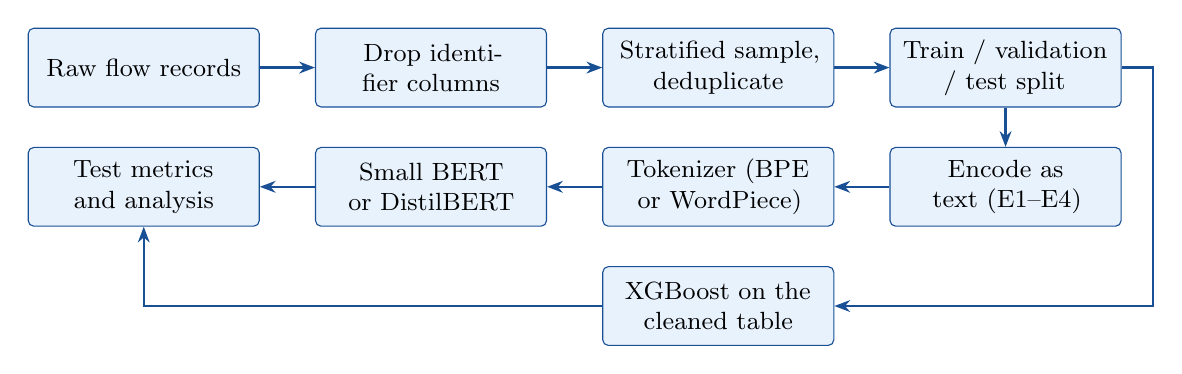
\begin{tikzpicture}[node distance=5mm and 7mm,
      box/.style={draw=accent, fill=accentlight!45, rounded corners=2pt, align=center, font=\small,
                  minimum height=10mm, text width=27mm},
      arr/.style={-{Stealth[length=2mm]}, accent, thick}]
    \node[box] (raw) {Raw flow records};
    \node[box, right=of raw] (clean) {Drop identifier columns};
    \node[box, right=of clean] (dedup) {Stratified sample, deduplicate};
    \node[box, right=of dedup] (split) {Train / validation / test split};
    \node[box, below=of split] (enc) {Encode as text (E1--E4)};
    \node[box, left=of enc] (tok) {Tokenizer (BPE or WordPiece)};
    \node[box, left=of tok] (lm) {Small BERT or DistilBERT};
    \node[box, left=of lm] (eval) {Test metrics and analysis};
    \node[box, below=of tok] (xgb) {XGBoost on the cleaned table};
    \draw[arr] (raw) -- (clean);
    \draw[arr] (clean) -- (dedup);
    \draw[arr] (dedup) -- (split);
    \draw[arr] (split) -- (enc);
    \draw[arr] (enc) -- (tok);
    \draw[arr] (tok) -- (lm);
    \draw[arr] (lm) -- (eval);
    \draw[arr] (split.east) -- ++(4mm,0) |- (xgb.east);
    \draw[arr] (xgb.west) -| (eval.south);
  \end{tikzpicture}
  \caption{Appendix A. Pipeline. Bin edges and tokenizers are fitted on the training split only, and the test split is read
    once.}
  \label{fig:pipeline}
\end{figure}

\clearpage
\section{Additional results}\label{app:more}
\Cref{tab:side} compares DistilBERT's truncated hash encodings with shorter hashes that fit its input limit
(\cref{sec:method}). \Cref{fig:exp2} shows the within-dataset macro-F1 of \cref{tab:exp2} as a chart, and
\cref{tab:accuracy} gives the within-dataset test accuracy, for comparison with the SecurityBERT paper. For the
cross-dataset runs of Experiment 3, \cref{fig:exp3} shows every train/test pair and \cref{fig:offdiag} summarises
the off-diagonal scores per method.

\begin{table}[H]
  \centering
  \caption{Appendix B. DistilBERT side runs: shorter hashes (nothing truncated) vs.\ the main runs, which are truncated to the
    model's input limit.}
  \label{tab:side}
  \gentable{exp2_side_runs}
\end{table}

\begin{figure}[H]
  \centering
  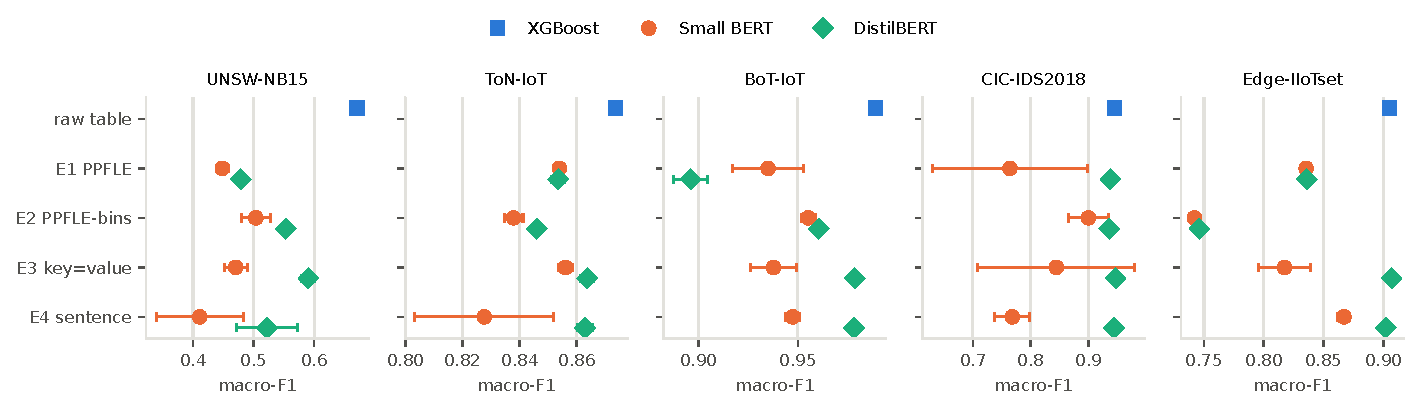
\includegraphics[width=\linewidth]{exp2_within_macro_f1}
  \caption{Appendix B. Within-dataset macro-F1 per encoding and model (bars: std over seeds). Each panel has
    its own x-range.}
  \label{fig:exp2}
\end{figure}

\begin{table}[H]
  \centering
  \caption{Appendix B. Test accuracy (multiclass), for comparison with the SecurityBERT paper.}
  \label{tab:accuracy}
  \gentable{exp2_within_accuracy}
\end{table}

\begin{figure}[H]
  \centering
  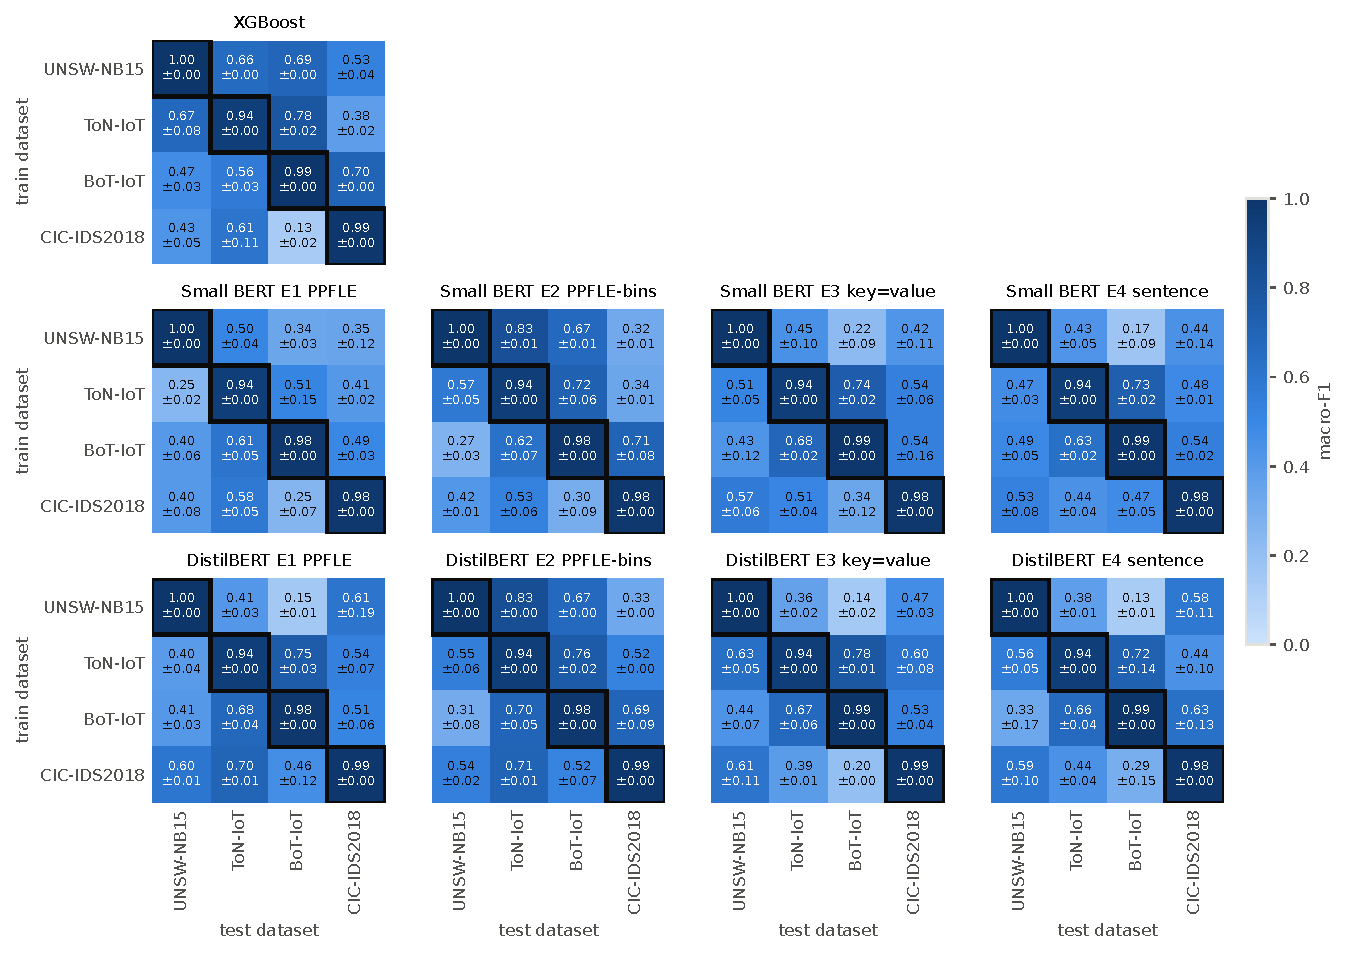
\includegraphics[width=\linewidth]{exp3_heatmaps_grid}
  \caption{Appendix B. Binary macro-F1, trained on the row dataset and tested on the column dataset (diagonal outlined).}
  \label{fig:exp3}
\end{figure}

\begin{figure}[H]
  \centering
  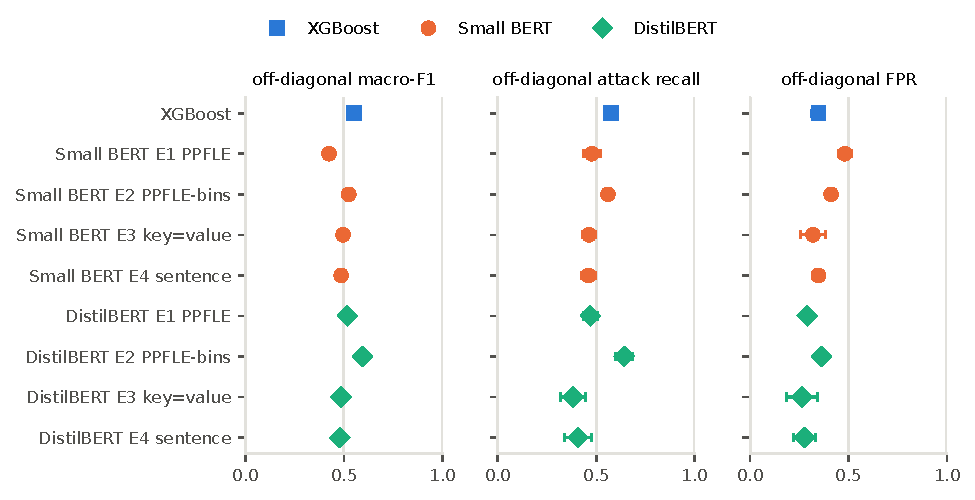
\includegraphics[width=0.85\linewidth]{exp3_offdiag}
  \caption{Appendix B. Off-diagonal macro-F1, attack recall and FPR per method.}
  \label{fig:offdiag}
\end{figure}

\clearpage
\section{Error analysis}\label{app:errors}
There is one figure per dataset (\cref{app:errors-unsw,app:errors-ton,app:errors-bot,app:errors-cic,app:errors-edge}).
In each figure, the top panel shows the per-class F1 of every method (mean over seeds). The bottom panel shows
confusion matrices for XGBoost and for the best encoding of each language model, as the share of each true class.

\subsection{NF-UNSW-NB15}\label{app:errors-unsw}
\begin{figure}[H]
  \centering
  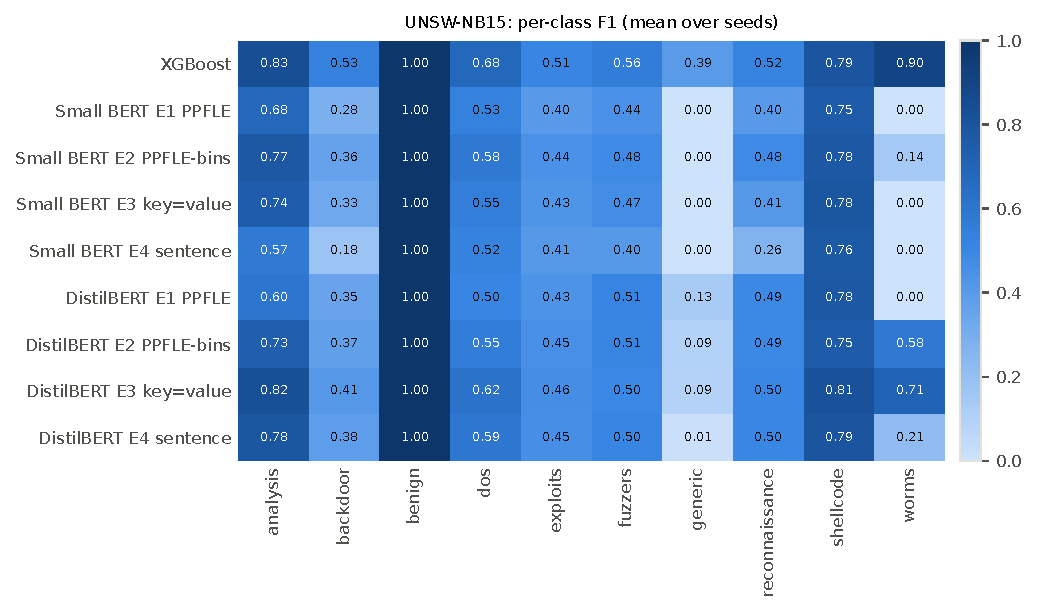
\includegraphics[width=\linewidth]{perclass_f1_nf_unsw_nb15}
  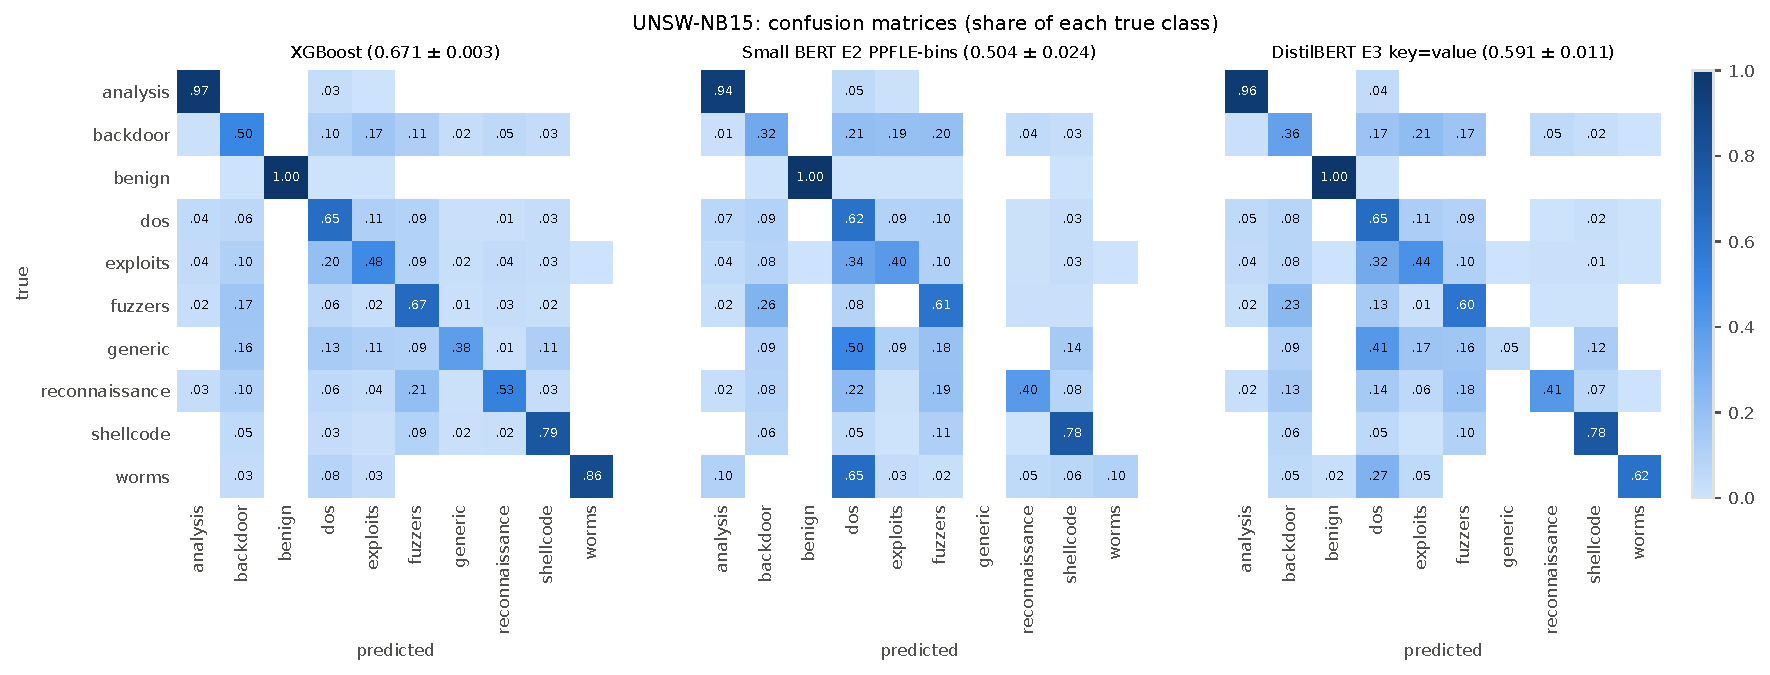
\includegraphics[width=\linewidth]{confusion_nf_unsw_nb15}
  \caption{Appendix C. Error analysis, NF-UNSW-NB15: per-class F1 (top) and confusion matrices (bottom).}
\end{figure}

\subsection{NF-ToN-IoT}\label{app:errors-ton}
\begin{figure}[H]
  \centering
  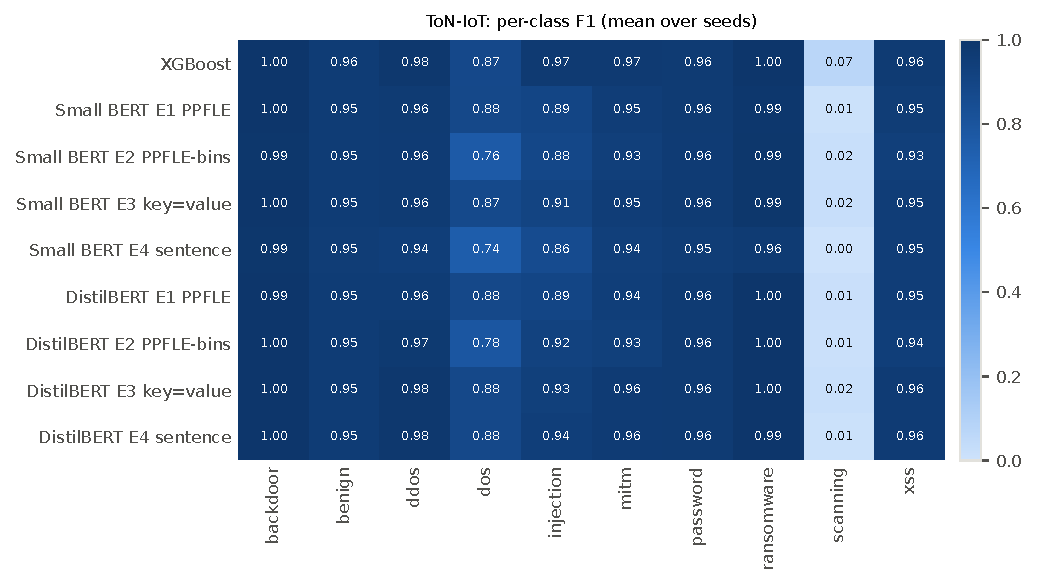
\includegraphics[width=\linewidth]{perclass_f1_nf_ton_iot}
  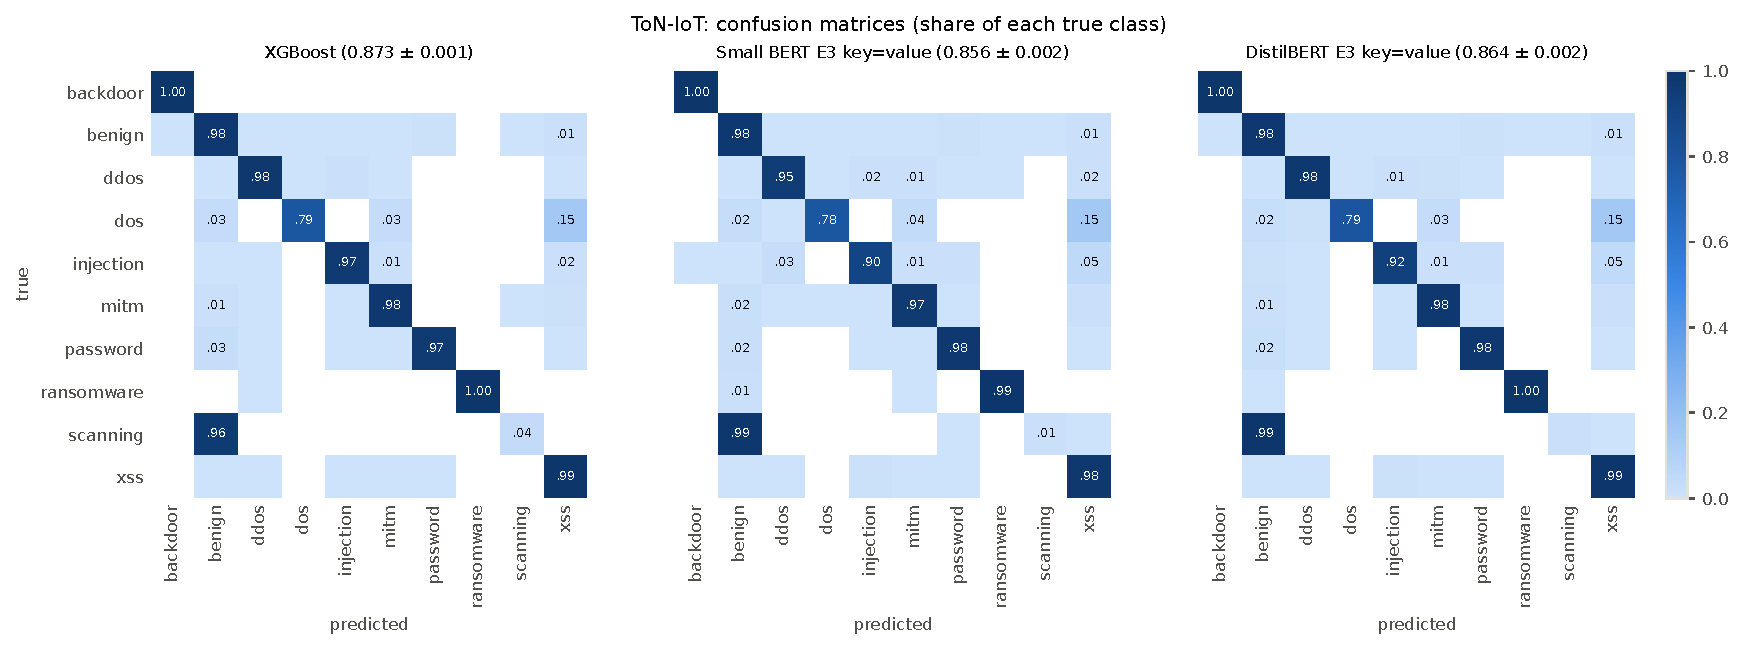
\includegraphics[width=\linewidth]{confusion_nf_ton_iot}
  \caption{Appendix C. Error analysis, NF-ToN-IoT: per-class F1 (top) and confusion matrices (bottom).}
\end{figure}

\subsection{NF-BoT-IoT}\label{app:errors-bot}
\begin{figure}[H]
  \centering
  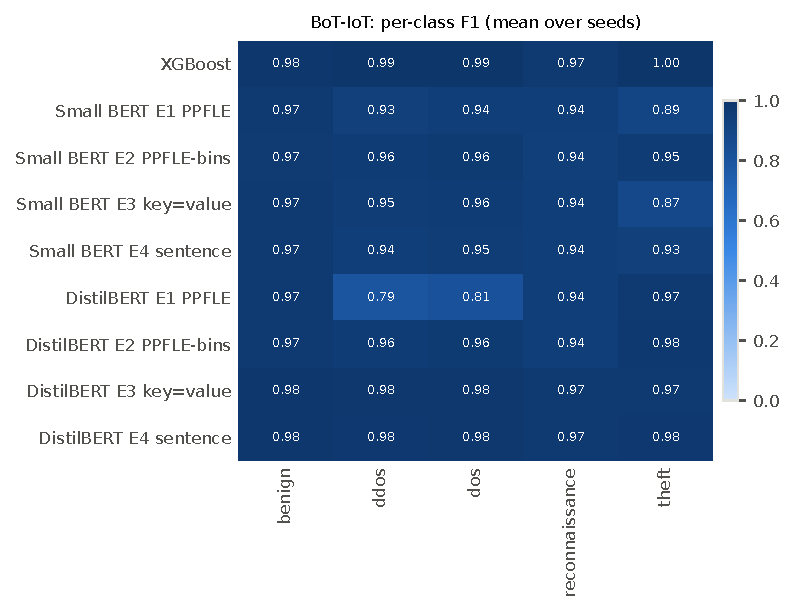
\includegraphics[width=\linewidth]{perclass_f1_nf_bot_iot}
  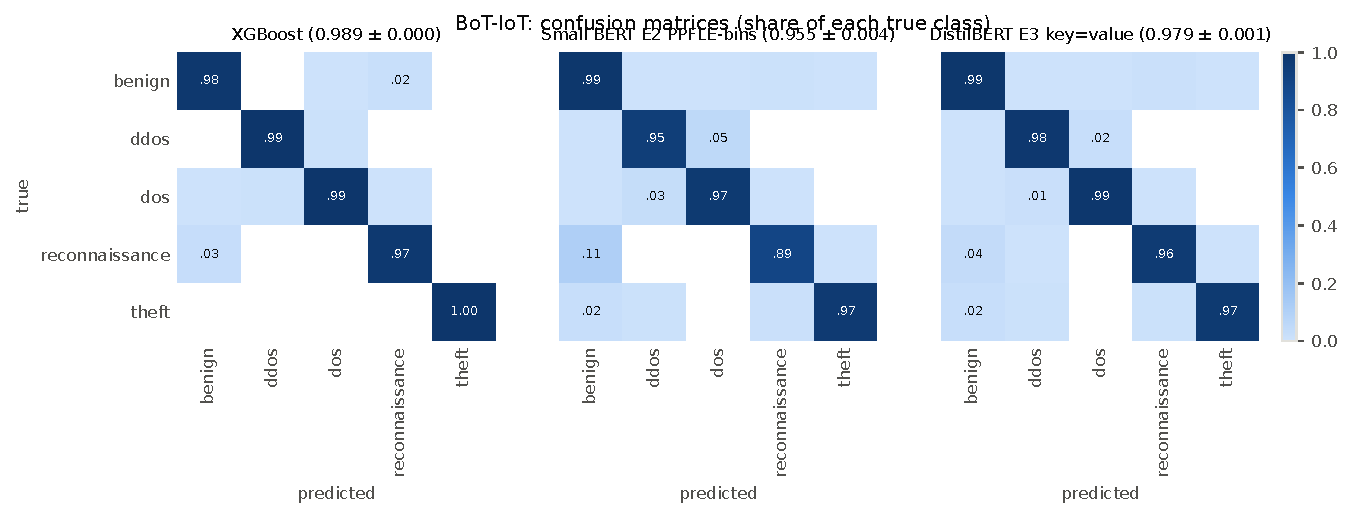
\includegraphics[width=\linewidth]{confusion_nf_bot_iot}
  \caption{Appendix C. Error analysis, NF-BoT-IoT: per-class F1 (top) and confusion matrices (bottom).}
\end{figure}

\subsection{NF-CSE-CIC-IDS2018}\label{app:errors-cic}
\begin{figure}[H]
  \centering
  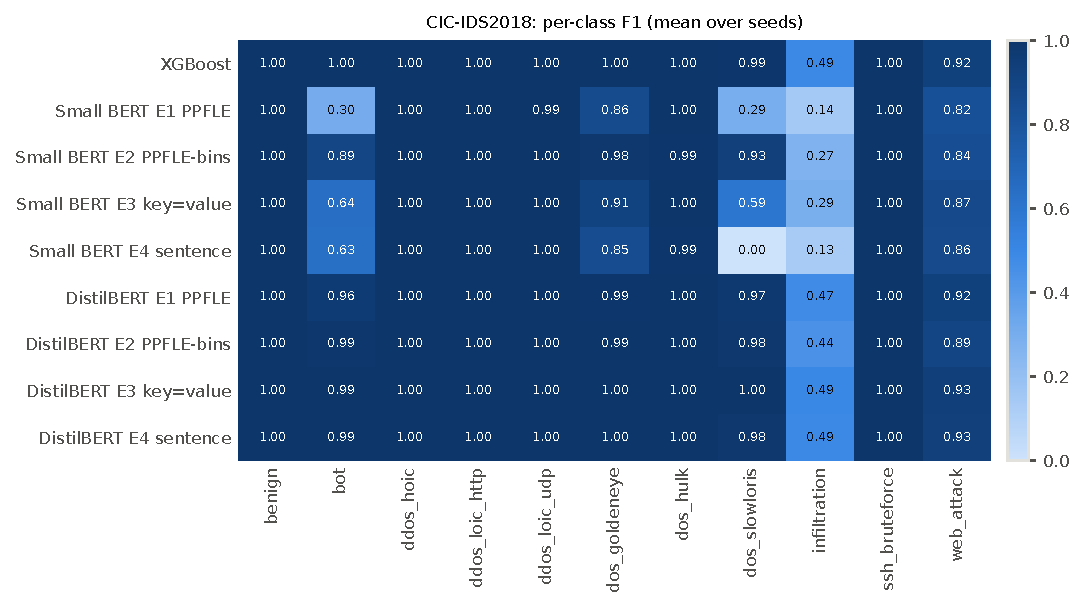
\includegraphics[width=\linewidth]{perclass_f1_nf_cse_cic_ids2018}
  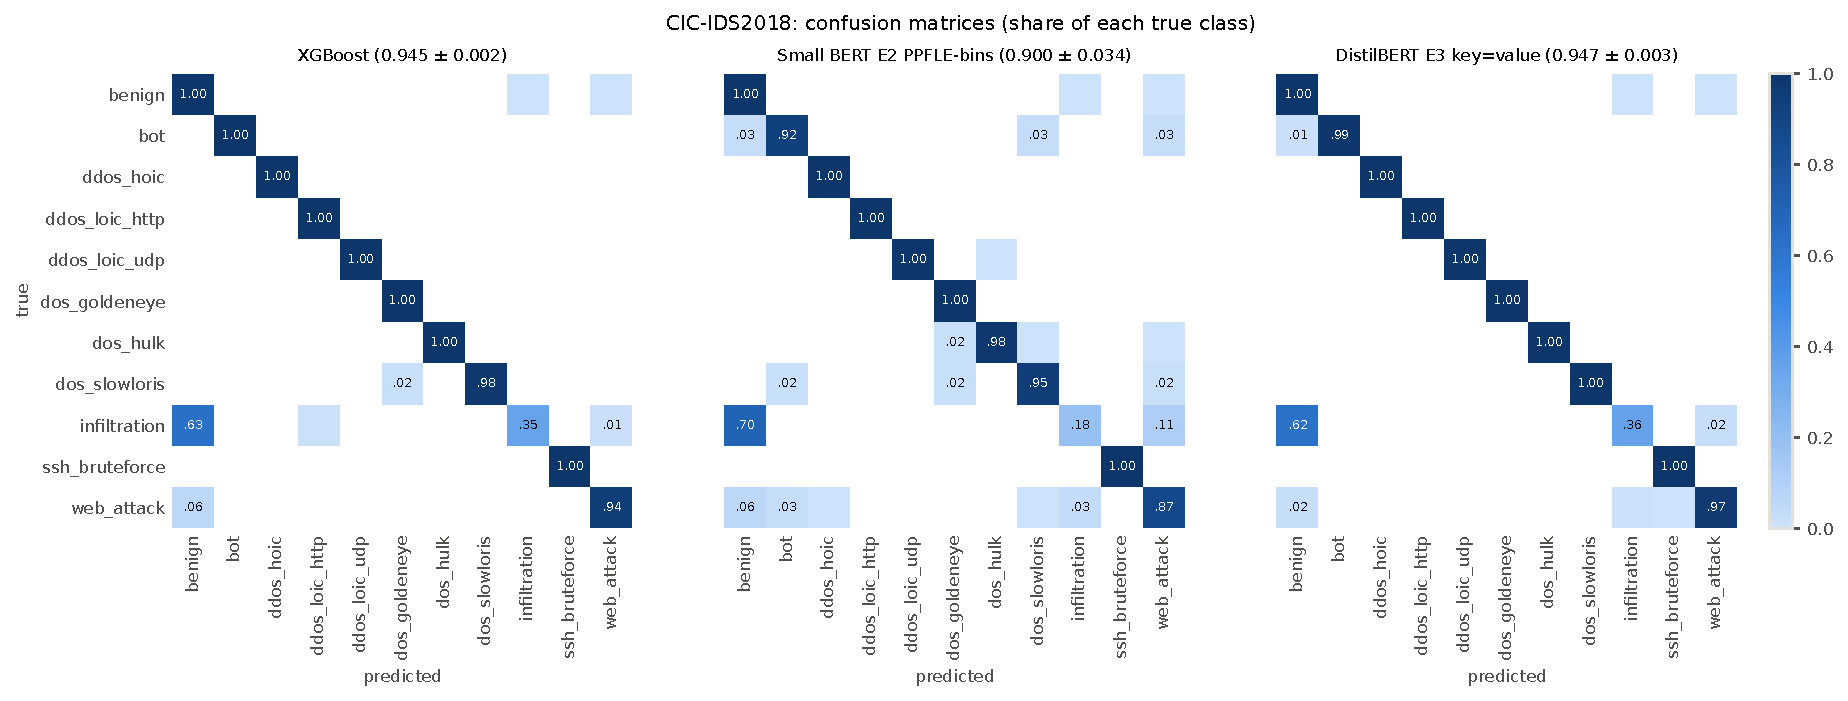
\includegraphics[width=\linewidth]{confusion_nf_cse_cic_ids2018}
  \caption{Appendix C. Error analysis, NF-CSE-CIC-IDS2018: per-class F1 (top) and confusion matrices (bottom).}
\end{figure}

\subsection{Edge-IIoTset}\label{app:errors-edge}
\begin{figure}[H]
  \centering
  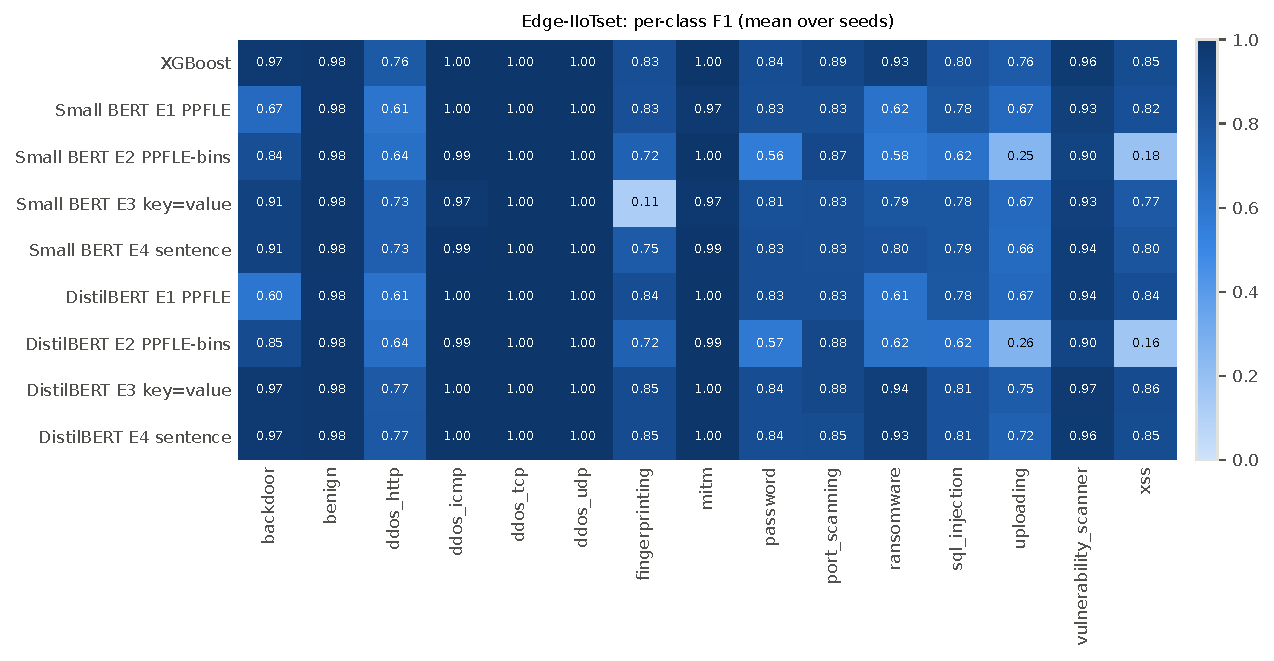
\includegraphics[width=\linewidth]{perclass_f1_edge_iiotset}
  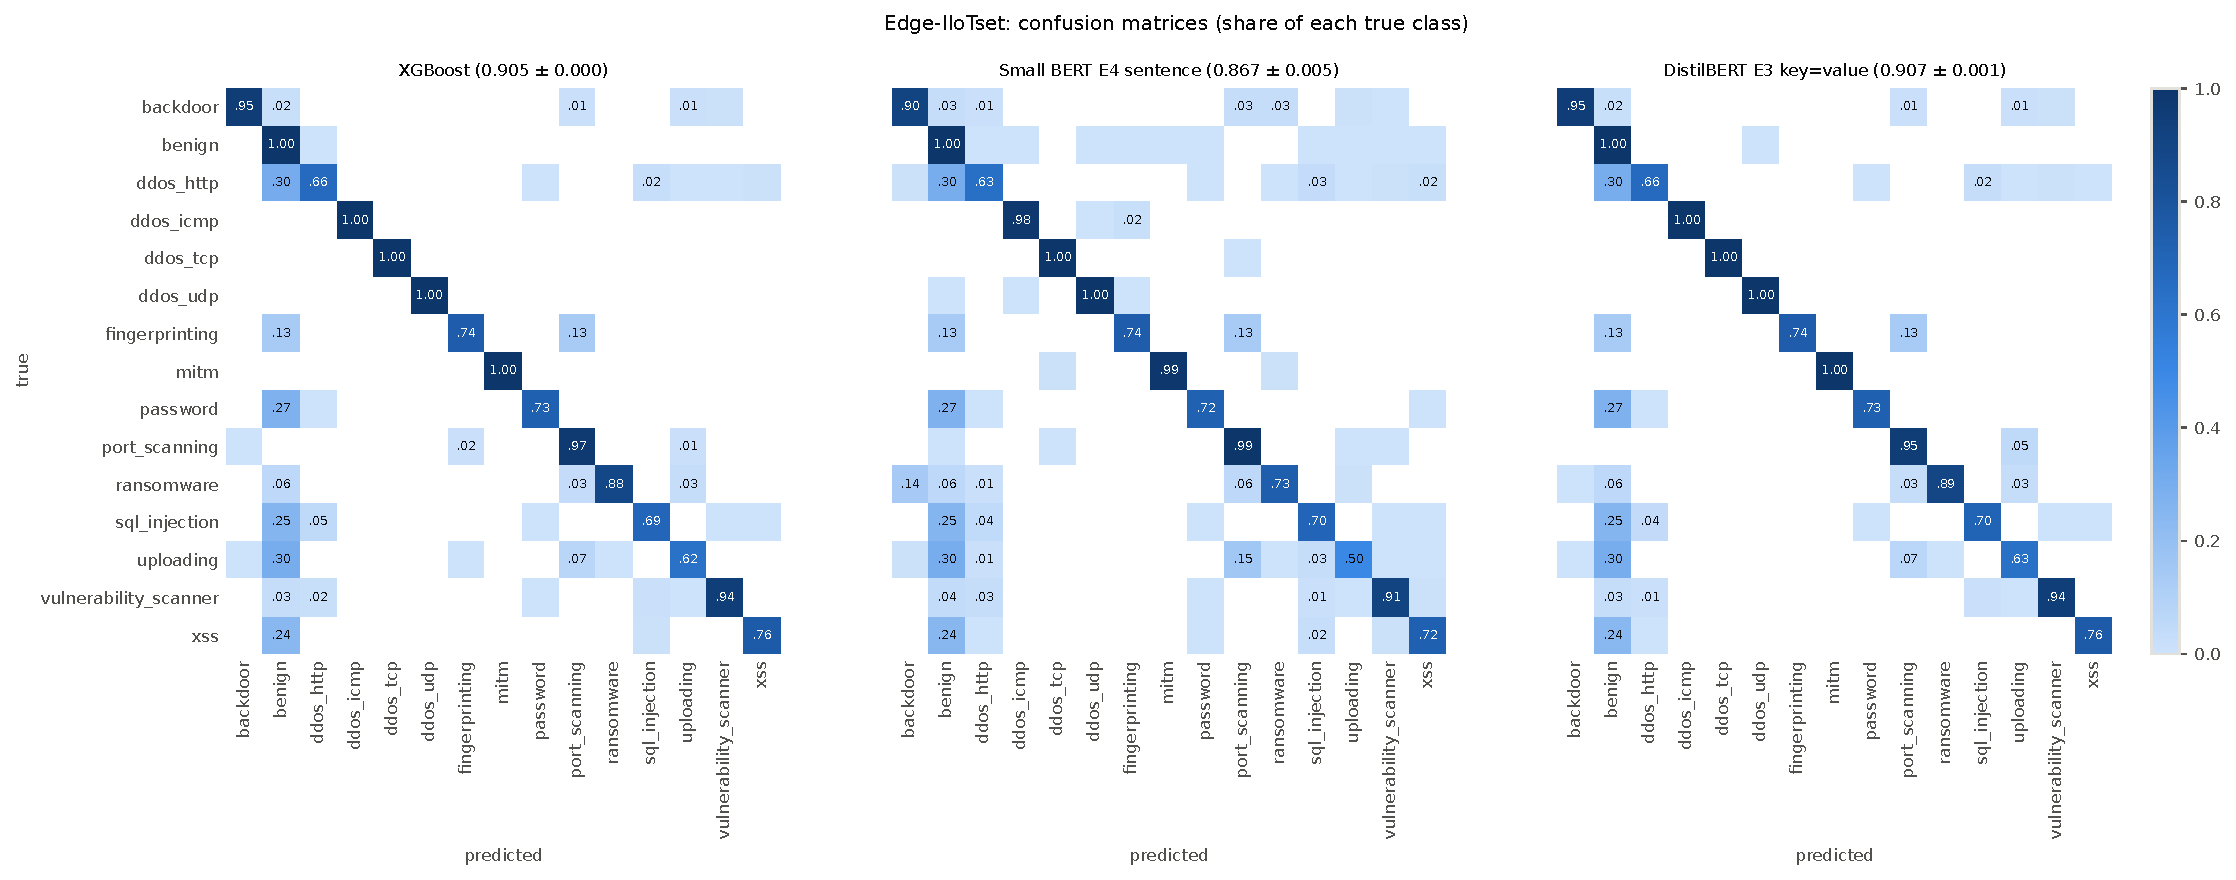
\includegraphics[width=\linewidth]{confusion_edge_iiotset}
  \caption{Appendix C. Error analysis, Edge-IIoTset (fixed data): per-class F1 (top) and confusion matrices (bottom).}
\end{figure}

\clearpage
\section{Privacy attack: further results}\label{app:privacy}
\Cref{fig:privacy} shows the share of NetFlow PPFLE tokens that each level of the dictionary attack of
Experiment 4 reverses, and \cref{tab:privacyedge} gives the attack on Edge-IIoTset. The share of test tokens
recovered per column is in \cref{fig:privacycols} for the NetFlow datasets and in \cref{fig:privacycolsedge} for
Edge-IIoTset.

\begin{figure}[H]
  \centering
  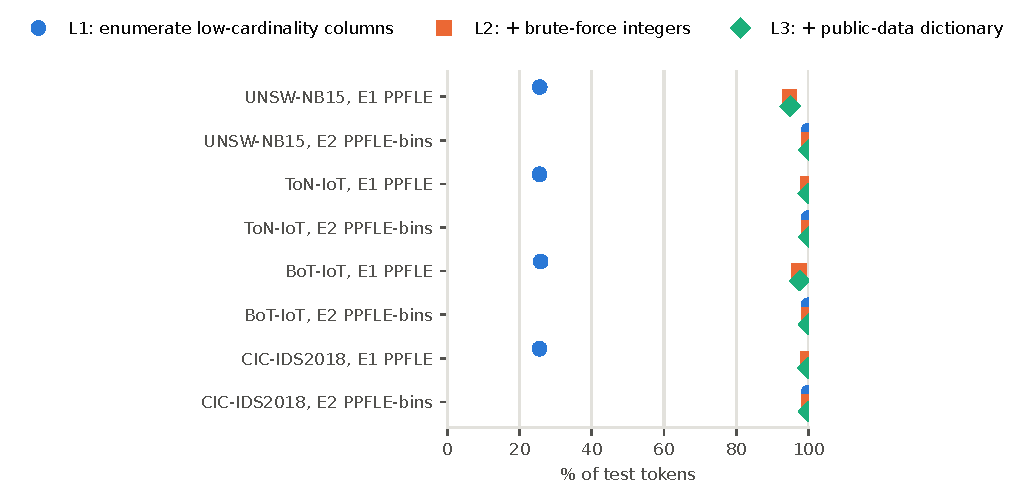
\includegraphics[width=0.8\linewidth]{privacy_attack_overall}
  \caption{Appendix D. Share of PPFLE test tokens reversed per attack level (NetFlow).}
  \label{fig:privacy}
\end{figure}

\begin{table}[H]
  \centering
  \caption{Appendix D. Dictionary attack on Edge-IIoTset (test split), levels L1 and L2.}
  \label{tab:privacyedge}
  \gentable{privacy_attack_edge}
\end{table}

\begin{figure}[H]
  \centering
  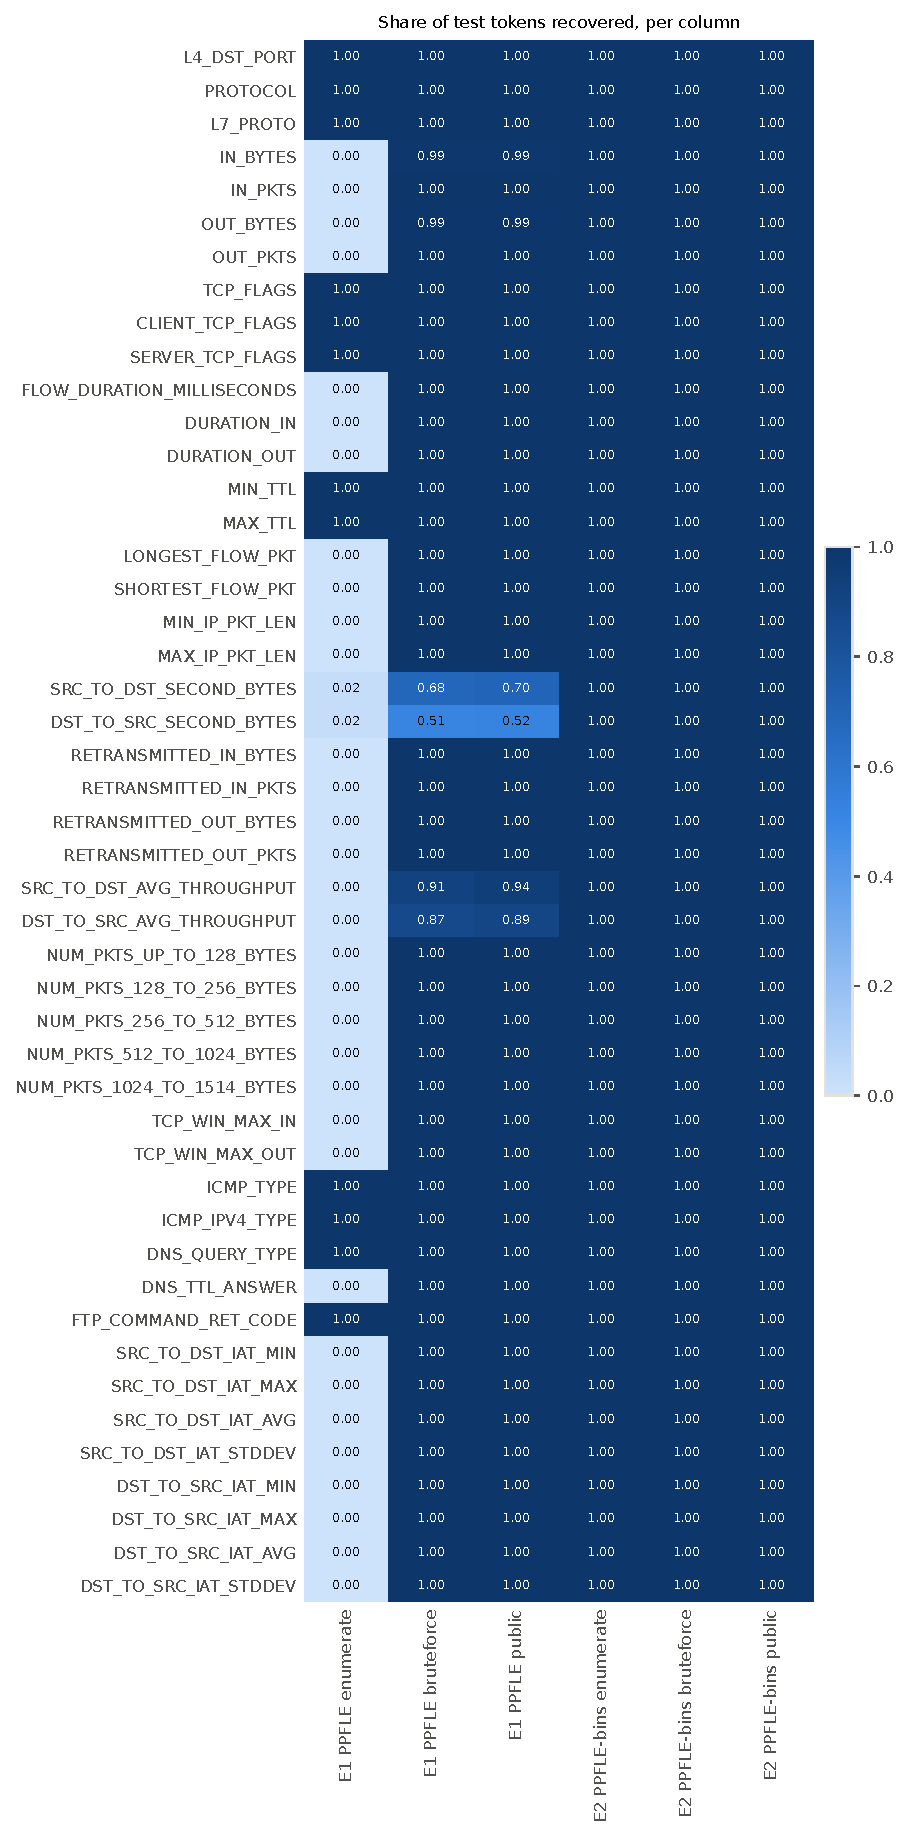
\includegraphics[height=0.75\textheight]{privacy_attack_columns}
  \caption{Appendix D. Privacy attack per column, NetFlow: share of test tokens recovered (pooled over datasets).}
  \label{fig:privacycols}
\end{figure}

\begin{figure}[H]
  \centering
  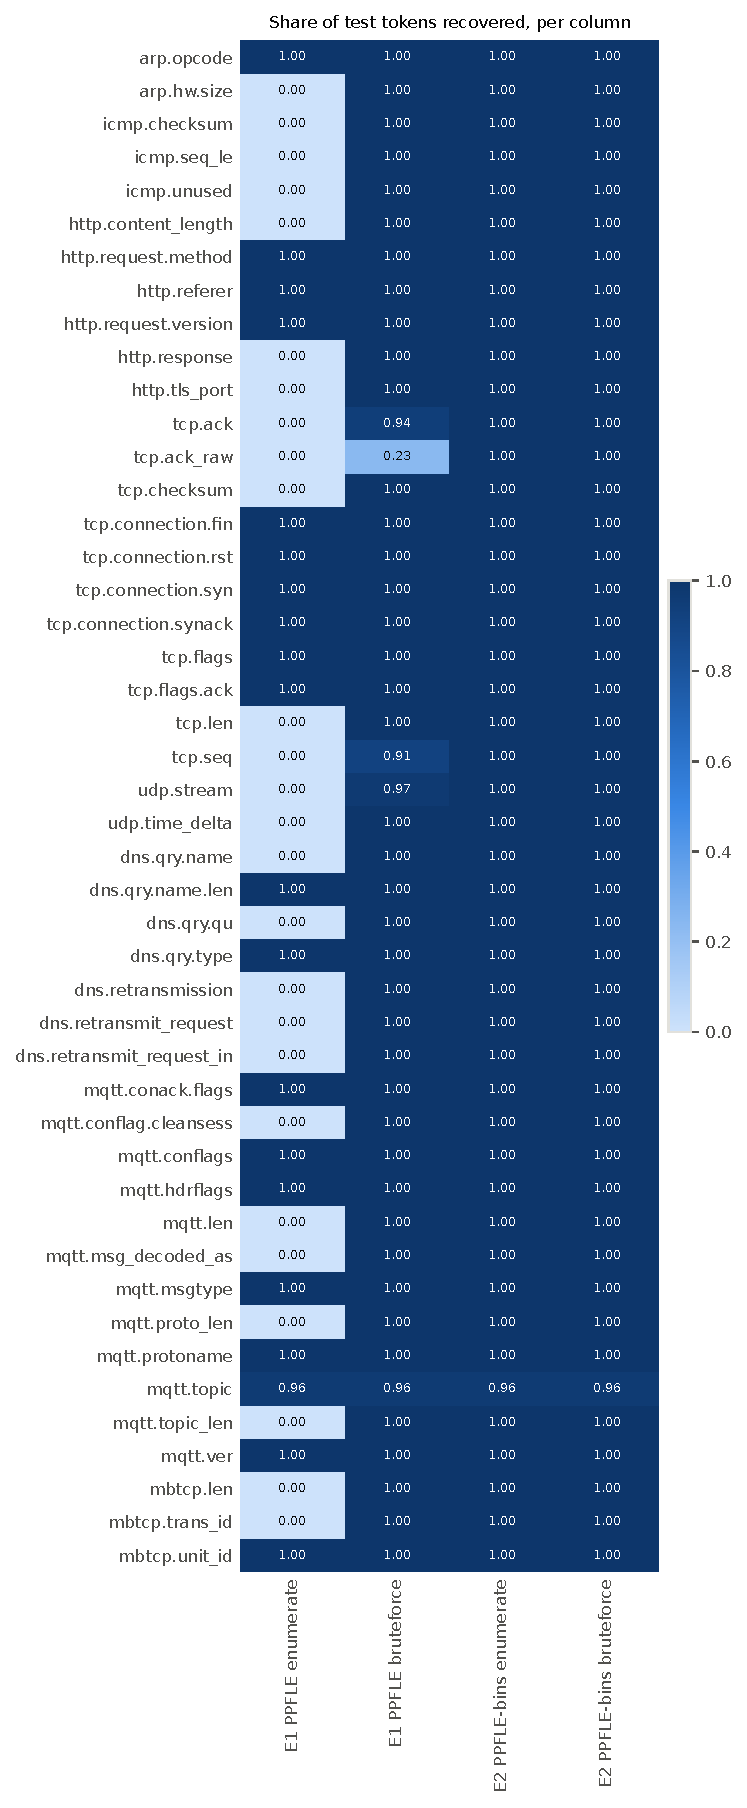
\includegraphics[height=0.75\textheight]{privacy_attack_edge_columns}
  \caption{Appendix D. Privacy attack per column, Edge-IIoTset: share of test tokens recovered (both versions pooled).}
  \label{fig:privacycolsedge}
\end{figure}

\end{document}
